
\documentclass[11pt,compress,t,notes=noshow, xcolor=table]{beamer}
\usepackage[]{graphicx}\usepackage[]{color}
% maxwidth is the original width if it is less than linewidth
% otherwise use linewidth (to make sure the graphics do not exceed the margin)
\makeatletter
\def\maxwidth{ %
  \ifdim\Gin@nat@width>\linewidth
    \linewidth
  \else
    \Gin@nat@width
  \fi
}
\makeatother

\definecolor{fgcolor}{rgb}{0.345, 0.345, 0.345}
\newcommand{\hlnum}[1]{\textcolor[rgb]{0.686,0.059,0.569}{#1}}%
\newcommand{\hlstr}[1]{\textcolor[rgb]{0.192,0.494,0.8}{#1}}%
\newcommand{\hlcom}[1]{\textcolor[rgb]{0.678,0.584,0.686}{\textit{#1}}}%
\newcommand{\hlopt}[1]{\textcolor[rgb]{0,0,0}{#1}}%
\newcommand{\hlstd}[1]{\textcolor[rgb]{0.345,0.345,0.345}{#1}}%
\newcommand{\hlkwa}[1]{\textcolor[rgb]{0.161,0.373,0.58}{\textbf{#1}}}%
\newcommand{\hlkwb}[1]{\textcolor[rgb]{0.69,0.353,0.396}{#1}}%
\newcommand{\hlkwc}[1]{\textcolor[rgb]{0.333,0.667,0.333}{#1}}%
\newcommand{\hlkwd}[1]{\textcolor[rgb]{0.737,0.353,0.396}{\textbf{#1}}}%
\let\hlipl\hlkwb

\usepackage{framed}
\makeatletter
\newenvironment{kframe}{%
 \def\at@end@of@kframe{}%
 \ifinner\ifhmode%
  \def\at@end@of@kframe{\end{minipage}}%
  \begin{minipage}{\columnwidth}%
 \fi\fi%
 \def\FrameCommand##1{\hskip\@totalleftmargin \hskip-\fboxsep
 \colorbox{shadecolor}{##1}\hskip-\fboxsep
     % There is no \\@totalrightmargin, so:
     \hskip-\linewidth \hskip-\@totalleftmargin \hskip\columnwidth}%
 \MakeFramed {\advance\hsize-\width
   \@totalleftmargin\z@ \linewidth\hsize
   \@setminipage}}%
 {\par\unskip\endMakeFramed%
 \at@end@of@kframe}
\makeatother

\definecolor{shadecolor}{rgb}{.97, .97, .97}
\definecolor{messagecolor}{rgb}{0, 0, 0}
\definecolor{warningcolor}{rgb}{1, 0, 1}
\definecolor{errorcolor}{rgb}{1, 0, 0}
\newenvironment{knitrout}{}{} % an empty environment to be redefined in TeX

\usepackage{alltt}
\newcommand{\SweaveOpts}[1]{}  % do not interfere with LaTeX
\newcommand{\SweaveInput}[1]{} % because they are not real TeX commands
\newcommand{\Sexpr}[1]{}       % will only be parsed by R
\newcommand{\xmark}{\ding{55}}%


\usepackage[english]{babel}
\usepackage[utf8]{inputenc}

\usepackage{dsfont}
\usepackage{verbatim}
\usepackage{amsmath}
\usepackage{amsfonts}
\usepackage{amssymb}
\usepackage{bm}
\usepackage{csquotes}
\usepackage{multirow}
\usepackage{longtable}
\usepackage{booktabs}
\usepackage{enumerate}
\usepackage[absolute,overlay]{textpos}
\usepackage{psfrag}
\usepackage{algorithm}
\usepackage{algpseudocode}
\usepackage{eqnarray}
\usepackage{arydshln}
\usepackage{tabularx}
\usepackage{placeins}
\usepackage{tikz}
\usepackage{setspace}
\usepackage{colortbl}
\usepackage{mathtools}
\usepackage{wrapfig}
\usepackage{bm}
\usepackage{amsmath}
\usepackage{pifont}
\usepackage{xcolor} %colored math symbols

\usetikzlibrary{shapes,arrows,automata,positioning,calc,chains,trees, shadows}
\tikzset{
  %Define standard arrow tip
  >=stealth',
  %Define style for boxes
  punkt/.style={
    rectangle,
    rounded corners,
    draw=black, very thick,
    text width=6.5em,
    minimum height=2em,
    text centered},
  % Define arrow style
  pil/.style={
    ->,
    thick,
    shorten <=2pt,
    shorten >=2pt,}
}

\usepackage{subfig}

% Defines macros and environments
\usepackage{../../style/lmu-lecture}


\let\code=\texttt
\let\proglang=\textsf

\setkeys{Gin}{width=0.9\textwidth}

\setbeamertemplate{frametitle}{\expandafter\uppercase\expandafter\insertframetitle}

\usepackage{bbm}
% basic latex stuff
\newcommand{\pkg}[1]{{\fontseries{b}\selectfont #1}} %fontstyle for R packages
\newcommand{\lz}{\vspace{0.5cm}} %vertical space
\newcommand{\dlz}{\vspace{1cm}} %double vertical space
\newcommand{\oneliner}[1] % Oneliner for important statements
{\begin{block}{}\begin{center}\begin{Large}#1\end{Large}\end{center}\end{block}}


%new environments
\newenvironment{vbframe}  %frame with breaks and verbatim
{
 \begin{frame}[containsverbatim,allowframebreaks]
}
{
\end{frame}
}

\newenvironment{vframe}  %frame with verbatim without breaks (to avoid numbering one slided frames)
{
 \begin{frame}[containsverbatim]
}
{
\end{frame}
}

\newenvironment{blocki}[1]   % itemize block
{
 \begin{block}{#1}\begin{itemize}
}
{
\end{itemize}\end{block}
}

\newenvironment{fragileframe}[2]{  %fragile frame with framebreaks
\begin{frame}[allowframebreaks, fragile, environment = fragileframe]
\frametitle{#1}
#2}
{\end{frame}}


\newcommand{\myframe}[2]{  %short for frame with framebreaks
\begin{frame}[allowframebreaks]
\frametitle{#1}
#2
\end{frame}}

\newcommand{\remark}[1]{
  \textbf{Remark:} #1
}


\newenvironment{deleteframe}
{
\begingroup
\usebackgroundtemplate{
\includegraphics[width=\paperwidth,height=\paperheight]{../style/color/red.png}}
 \begin{frame}
}
{
\end{frame}
\endgroup
}
\newenvironment{simplifyframe}
{
\begingroup
\usebackgroundtemplate{
\includegraphics[width=\paperwidth,height=\paperheight]{../style/color/yellow.png}}
 \begin{frame}
}
{
\end{frame}
\endgroup
}\newenvironment{draftframe}
{
\begingroup
\usebackgroundtemplate{
\includegraphics[width=\paperwidth,height=\paperheight]{../style/color/green.jpg}}
 \begin{frame}
}
{
\end{frame}
\endgroup
}
% https://tex.stackexchange.com/a/261480: textcolor that works in mathmode
\makeatletter
\renewcommand*{\@textcolor}[3]{%
  \protect\leavevmode
  \begingroup
    \color#1{#2}#3%
  \endgroup
}
\makeatother


\input{../../latex-math/basic-math}
\input{../../latex-math/basic-ml}
\input{../../latex-math/ml-nn}

\newcommand{\titlefigure}{figure/backprop_gg_new.png}
\newcommand{\learninggoals}{
  \item Chain rule of calculus
  \item Computational graphs
}

\title{Deep Learning}
\date{}

\begin{document}

\lecturechapter{Chain Rule and Computational Graphs}
\lecture{I2DL}

%%%%%%%%%%%%%%%%%%%%%%%%%%%%%%%%%%%%%%%%%%%%%%%%%%%%%%%%%%%%%%%%%%

%\begin{frame}
%\frametitle{Lecture outline}
%\tableofcontents
%\end{frame}
%%%%%%%%%%%%%%%%%%%%%%%%%%%%%%%%%%%%%%%%%%%%%%%%%%%%%%%%%%%%%%%%%%
% \begin{frame}{Local Minima/Convexity}
% \end{frame}

% \section{Chain Rule and Computational Graphs}
%%%%%%%%%%%%%%%%%%%%%%%%%%%%%%%%%%%%%%%%%%%%%%%%%%%%%%%%%%%%%%%%%%
\begin{vbframe}{Chain rule of calculus}
  % \begin{itemize}
  %   \item The chain rule can be used to compute derivatives of the composition of two or more functions.
  %   \item Let $x \in \R^m$, $y \in \R^n$, \\
  %         $g: \R^m \to \R^n$ and $f: \R^n \to \R$. \\
  %   \item If $y = g(x)$ and $z = f(y)$, the chain rule yields $$\frac{\partial z}{\partial x_i} = \sum_j \frac{\partial z}{\partial y_j} \frac{\partial y_j}{\partial x_i}$$
  %         or in vector notation $$\nabla_x z = \Big(\frac{\partial y}{\partial x}\Big)^\top \nabla_y z,$$
  %         where $\frac{\partial y}{\partial x}$ is the $n \times m$ jacobian matrix of $g$.
  % \end{itemize}
  \begin{itemize}
    \item The chain rule can be used to compute derivatives of the composition of two or more functions.
    \item Let $\xv \in \R^m$, $\mathbf{y} \in \R^n$, \\
          $g: \R^m \to \R^n$ and $f: \R^n \to \R$. \\
    \item If $\mathbf{y} = g(\xv)$ and $z = f(\mathbf{y})$, the chain rule yields: $$\frac{\partial z}{\partial x_i} = \sum_j \frac{\partial z}{\partial y_j} \cdot \frac{\partial y_j}{\partial x_i}$$
          or, in vector notation: $$\nabla_{\xv} z = \Big(\frac{\partial \mathbf{y}}{\partial \xv}\Big)^\top \nabla_{\mathbf{y}} z,$$
          where $\frac{\partial \mathbf{y}}{\partial \xv}$ is the ($n \times m$) Jacobian matrix of $g$.
  \end{itemize}
\end{vbframe}  

\begin{vbframe}{Computational graphs}
  \begin{minipage}{0.5\textwidth}
    \begin{itemize}
      \item CGs are nested expresssions, visualized as graphs.
      \item Each node is a variable, either an input or derived.
      \item Derived variables are functions applied to other variables.
    \end{itemize}
  \end{minipage}\hfill
  \begin{minipage}{0.5\textwidth}
    \begin{figure}
      \centering
        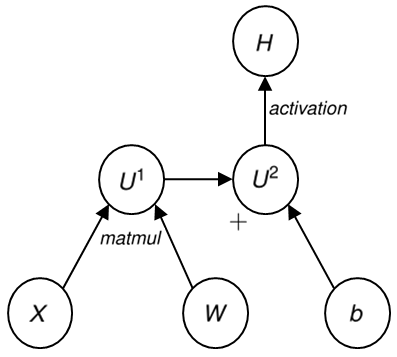
\includegraphics[width=6cm]{figure/compgraph1.png}
        \tiny{\\source : Goodfellow et al. (2016)}
        \caption{The computational graph for the expression $H = \sigma(XW + B)$ with activation function $\sigma(\cdot)$.}
    \end{figure}
  \end{minipage}  
\end{vbframe}

\begin{vbframe}{Chain rule of calculus: Example 1}
  \begin{minipage}{0.5\textwidth}
    \begin{itemize}
      \item Suppose we have the following computational graph.
      \item To compute the derivative of $\frac{\partial z}{\partial w}$ %$\frac{\partial z}{\partial w}$ 
      we need to recursively apply the chain rule. That is:
      \begin{eqnarray*}
        \frac{\partial z}{\partial w} &=& \frac{\partial z}{\partial y} \cdot \frac{\partial y}{\partial x} \cdot \frac{\partial x}{\partial w} \\
                                  &=& f'_3(y) \cdot f'_2(x) \cdot f'_1(w) \\
                                  &=& f'_3(f_2(f_1(w))) \cdot f'_2(f_1(w)) \cdot f'_1(w)
      \end{eqnarray*}
    \end{itemize}
  \end{minipage}\hfill
  \begin{minipage}{0.32\textwidth}
    \begin{figure}
      \centering
        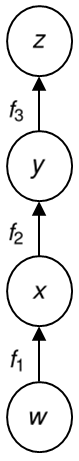
\includegraphics[width=1cm]{figure/compgraph2.png}
        \begin{footnotesize}
        \tiny{\\source : Goodfellow et al. (2016)}
        \caption{A computational graph, such that $x = f_1(w),$ $y = f_2(x)$ and $z = f_3(y)$.}
        \end{footnotesize}
    \end{figure}
  \end{minipage}
% \framebreak
%   \begin{figure}
%     \centering
%       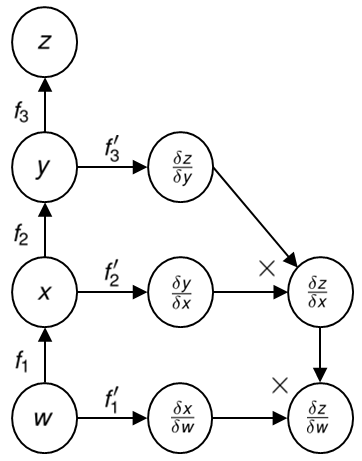
\includegraphics[width=4.5cm]{figure/compgraph3.png}
%       \caption{Applying the chain rule to the example yields us a computational graph with a symbolic description of the
% derivatives.}
%   \end{figure}  
\end{vbframe}

\begin{frame}{Chain rule of calculus: Example 2}

   \begin{figure}
    \centering
      \scalebox{0.27}{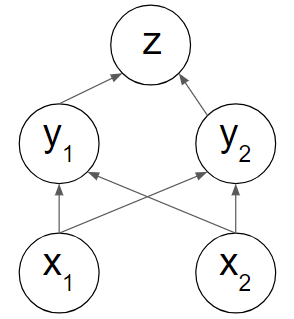
\includegraphics{figure/chain_tree.png}}
  \end{figure}
  
To compute $\nabla_\xv z$, we apply the chain rule % to the computational graph above,
  \begin{itemize}
    \item $\frac {\partial z}{\partial x_1} = \sum_j \frac{\partial z}{\partial y_j} \frac{\partial y_j}{\partial x_1} = \frac {\partial z}{\partial y_1} \frac {\partial y_1}{\partial x_1} + \frac {\partial z}{\partial y_2} \frac {\partial y_2}{\partial x_1}$
    \item $\frac {\partial z}{\partial x_2} = \sum_j \frac{\partial z}{\partial y_j} \frac{\partial y_j}{\partial x_2} = \frac {\partial z}{\partial y_1} \frac {\partial y_1}{\partial x_2} + \frac {\partial z}{\partial y_2} \frac {\partial y_2}{\partial x_2}$
  \end{itemize}
  \vspace{2mm}
    Therefore, the gradient of $z$ w.r.t $\xv$ is
    \begin{itemize}
      \item  $\nabla_\xv z = \begin{bmatrix}
               \frac {\partial z}{\partial x_1} \\
               \frac {\partial z}{\partial x_2} \\
             \end{bmatrix} = \underbrace{\begin{bmatrix} \frac{\partial y_1}{\partial x_1}&\frac {\partial y_2}{\partial x_1}\\
                                             \frac {\partial y_1}{\partial x_2}&\frac {\partial y_2}{\partial x_2}\\
             \end{bmatrix}}_{\textcolor{red}{(\frac{\partial \mathbf{y}}{\partial \xv})^\top}} \underbrace{\begin{bmatrix} \frac {\partial z}{\partial y_1} \\
            \frac {\partial z}{\partial y_2} \\ \end{bmatrix}}_{\textcolor{red}{\nabla_{\mathbf{y}} z}} = \Big(\frac{\partial \mathbf{y}}{\partial \xv}\Big)^\top \nabla_{\mathbf{y}} z $
  \end{itemize}
\end{frame}

\begin{frame} {Computational Graph: Neural Net}
  \begin{figure}
      \centering
        \scalebox{0.75}{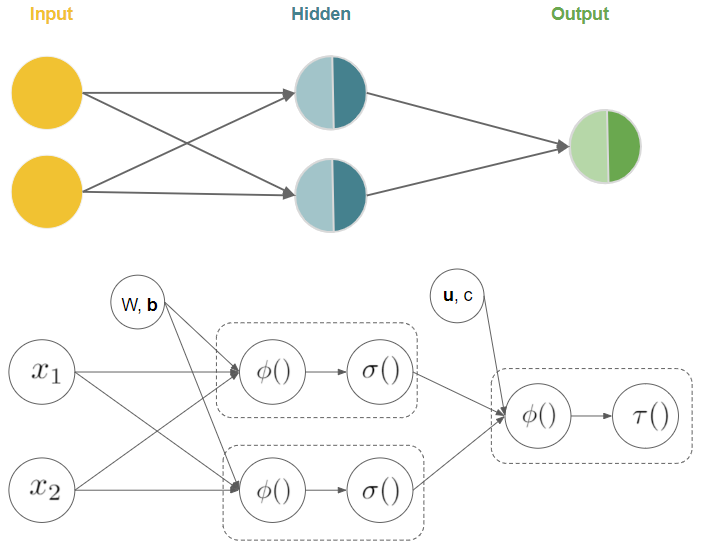
\includegraphics{figure/neo_comp.png}}
        \caption{A neural network can be seen as a computational graph. $\phi$ is the weighted sum and $\sigma$ and $\tau$ are the activations. \\
        Note: In contrast to the top figure, the arrows in the computational graph below merely indicate \textbf{dependence}, not weights.}
    \end{figure}
\end{frame}
% \begin{frame}{Chain rule of calculus}
% \begin{figure}
%     \centering
%       \scalebox{0.4}{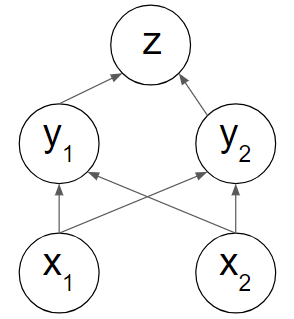
\includegraphics{figure/chain_tree.png}}
%   \end{figure}
%   
%     $\nabla_x z = \begin{bmatrix}
%            \frac {\partial z}{\partial x_1} \\
%            \frac {\partial z}{\partial x_2} \\
%          \end{bmatrix} = \begin{bmatrix}
%            \frac {\partial z}{\partial x_1} \\
%            \frac {\partial z}{\partial x_2} \\
%          \end{bmatrix}$
% \end{frame}


%%%%%%%%%%%%%%%%%%%%%%%%%%%%%%%%%%%%%%%%%%%%%%%%%%%%%%%%%%%%%%%%%%
%%%%%%%%%%%%%%%%%%%%%%%%%%%%%%%%%%%%%%%%%%%%%%%%%%%%%%%%%%%%%%%%%%
% \begin{frame} {Simple Example?}
%   \begin{figure}
%     \centering
%       \scalebox{1}{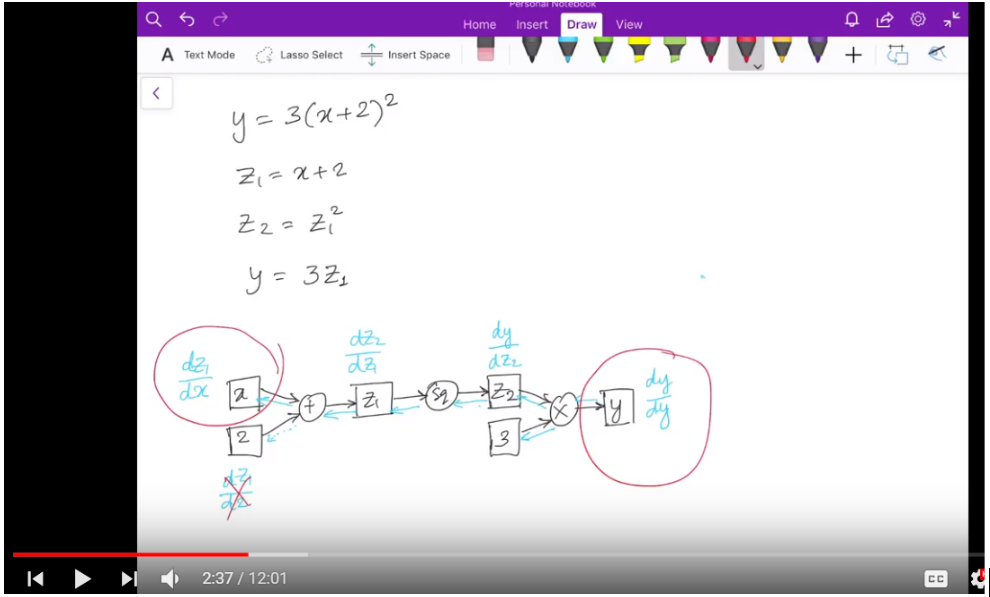
\includegraphics{figure/simex.png}}
%   \end{figure}
% \end{frame}
%%%%%%%%%%%%%%%%%%%%%%%%%%%%%%%%%%%%%%%%%%%%%%%%%%%%%%%%%%%%%%%%%%

%%%%%%%%%%%%%%%%%%%%%%%%%%%%%%%%%%%%%%%%%%%%%%%%%%%%%%%%%%%%%%%%%%
%%%%%%%%%%%%%%%%%%%%%%%%%%%%%%%%%%%%%%%%%%%%%%%%%%%%%%%%%%%%%%%%%%
%%%%%%%%%%%%%%%%%%          REFERENCES          %%%%%%%%%%%%%%%%%%
%%%%%%%%%%%%%%%%%%%%%%%%%%%%%%%%%%%%%%%%%%%%%%%%%%%%%%%%%%%%%%%%%%

%\section{References}

%\begin{vbframe}
%\frametitle{References}
%\footnotesize{
%\begin{thebibliography}{99}

%%%%%%%%%%%%%%%%%%%%%%%%%%%%%%%%%%%
%\bibitem[Ian Goodfellow et al., 2016]{1} Ian Goodfellow, Yoshua Bengio and Aaron Courville (2016)
%\newblock Deep Learning
%\newblock \emph{\url{http://www.deeplearningbook.org/}}
%%%%%%%%%%%%%%%%%%%%%%%%%%%%%%%%%%%

%\end{thebibliography}
%}
%\end{vbframe}
%%%%%%%%%%%%%%%%%%%%%%%%%%%%%%%%%%%%%%%%%%%%%%%%%%%%%%%%%%%%%%%%%%
%%%%%%%%%%%%%%%%%%%%%%%%%%%%%%%%%%%%%%%%%%%%%%%%%%%%%%%%%%%%%%%%%%

\endlecture
\end{document}
